Observa el siguiente termómetro que marca la temperatura en una mañana. Si durante la tarde la temperatura sube 7 grados y luego baja 4 grados en la noche, ¿cuál será la temperatura final?

\begin{center}
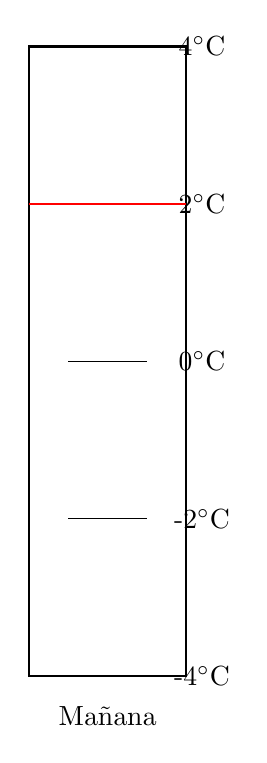
\begin{tikzpicture}
    \draw[thick] (0,0) rectangle (2,8);
    \foreach \y in {0,2,4,6,8} {
        \draw (0.5,\y) -- (1.5,\y);
        \pgfmathsetmacro{\temp}{int(\y-4)}
        \node at (2.2,\y) {\temp$^\circ$C};
    }
    % Marca inicial a 2°C (altura 6)
    \draw[red, thick] (0,6) -- (2,6);
    \node at (1, -0.5) {Mañana};
\end{tikzpicture}
\end{center}